

\begin{figure}

\centering
\begin{subfigure}{0.22\textwidth}

\includegraphics[width=\textwidth]{S12.eps}
\caption{}
\label{fig:figure1}
\end{subfigure}
\quad
\begin{subfigure}{0.22\textwidth}
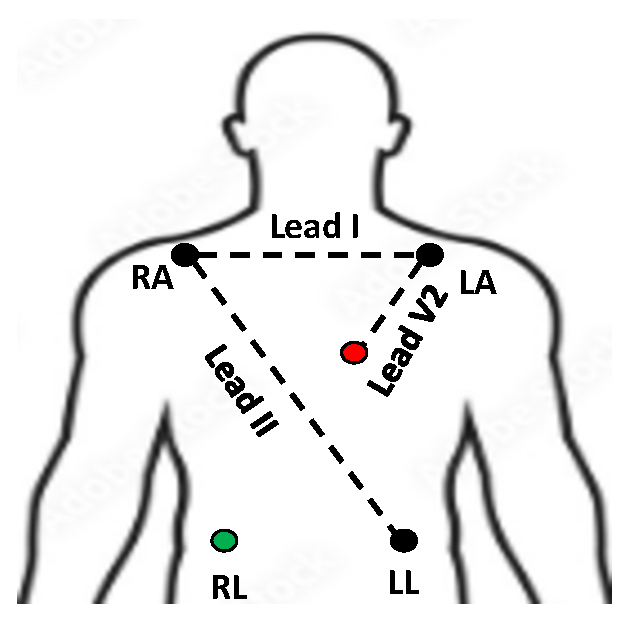
\includegraphics[width=\textwidth]{R3L.eps}
\caption{}
\label{fig:figure2}
\end{subfigure}

% \vspace{0cm} % Adjust the vertical space between the rows of figures
  
\begin{subfigure}{0.5\textwidth}
\centering

\includegraphics[width=0.6\textwidth]{3D.eps}
\caption{}
\label{fig:figure3}
\end{subfigure}

\caption{(a) Standard 12-Lead ECG system; (b) Reduced 3-Lead ECG system; (c) Schematic presentation of the lead vectors of Standard 12-lead ECG system with the 3 leads in the reduced system circled.}
\label{S12_R3L_3D}

\end{figure}